\section{Wechselrichter}
\subsection{Einphasig}
\textbf{Amplitudenmodulation}\newline
Um die Amplitude der Ausgangsspannung stufenlos zu verstellen, verwendet amn die \textbf{Pulsbreitenmodulation PWM}. \newline
Ist die Taktzahl ein ganzzahliges Vielfaches der Grundfrequenz, so spricht man von einer synchronen Taktung, ansonsten von einer asynchronen.
Bei Asynchroner Taktung treten Schwebungen der Grundfrequenz auf $ f_s = f_1 \pm f_T $ welche zusätzliche Verluste erteugen. Spätestens wenn die Taktdrequenz nur noch 10mal höher als die Grundfreq. ist muss auf Synchrone Taktung umgetsellt werden. \newline
\begin{tabular}{ p{.30\textwidth}  p{.2\textwidth} }
    Schalt oder Taktzahl&
    $ q = \frac{f_s}{f_1} $
    \\
    
    Schwebe-frequenz&
    $ f_s = f_1 \pm f_T $
    \\   
\end{tabular}

\textbf{Signalmodulation}\newline
Durch die PWM sind die ausganssignale Rechteck-förmig. Um Motoren optimal anzusteuern braucht es Sinusförmige Signale.\newline

\begin{tabular}{ p{.20\textwidth}  p{.3\textwidth} p{.4\textwidth}}
    Modulation&
    $$ m=M\cdot sin(\omega_1 \cdot t_1 \cdot \varphi_m) $$\newline
    $$  M= \frac{\hat{u}_{U0,1}}{\frac{U_D}{2}} =\frac{\hat{u}_{U0,1}}{u_{U0,1}} $$&
    m= Modulationsfunktion\newline
    M= Modulationsgrad\newline
    $ \varphi_m $= Phasenverschiebung der Grundfreq\newline
    $ \omega_1 $= Kreisfreq der Grundfreq $ f_1 $
    \\
    
    Aussteuerungsgrad&
    $$A = \frac{\hat{u}_{U0,1}}{\frac{2}{\pi}U_D\sqrt{3}} $$&
    $ 0\leq A \leq 1 $\newline
    $ A_{max}=\frac{\pi}{4} $
    \\   
\end{tabular}

\textbf{Übung 7 Einphasiger Wechselrichter}\newline
\begin{tabular}{ p{.30\textwidth}  p{.2\textwidth} }       
        $\tau = \frac{L}{R} \qquad T = \frac{1}{f} \qquad \diff t = \frac{T}{N-1}$ \newline\newline&
        \\
            
        \textbf{Schaltzeitpunkte}&\\              
        $t_e(i) = (i-1) \cdot \diff t$\newline
        $t_a(i) = t_e(i) + k \cdot \diff t \cdot |\sin(\omega \cdot t_e(i))|$\newline\newline&
        \\
       
        \textbf{Laststrom} & \\          
        $i_L(t) = \frac{U_1}{R} \cdot \left( 1-e^{\frac{t_{ei}-t}{\tau}}\right) + i_L(t_{ei}) \cdot e^{\frac{t_{ei}-t}{\tau}}$&
        $t \in [t_{ei},t_{ai}]$
        \\
                  
        $i_L(t) = i_L(t_{ai}) \cdot e^{\frac{t_{ai}-t}{\tau}}$&
        $t \in [t_{ai},t_{ei+1}]$
        \\
\end{tabular}
\begin{minipage}{0.5\linewidth}
        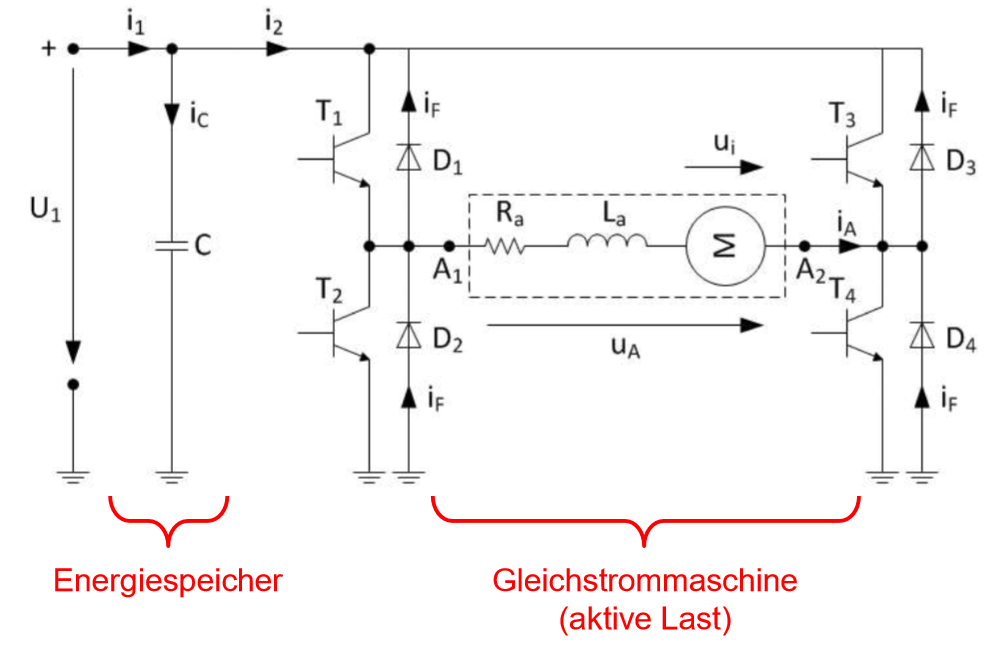
\includegraphics[width=0.9\linewidth]{images/WrEinphaseSchema}\newline
        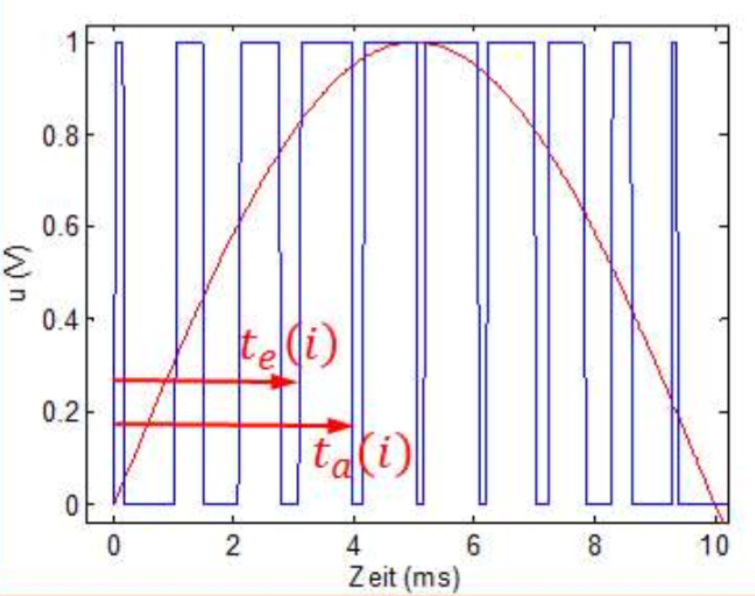
\includegraphics[width=0.5\linewidth]{images/WrEinphaseTime}
\end{minipage}
\clearpage